\section{User Study Evaluation}
We ran the study between \textcolor{red}{begin and end date} in Huxley 218 on the Imperial College London South Kensington Campus. In the end we managed to collect \textcolor{red}{16?} participants.

\textcolor{red}{INSERT DIAGRAM HERE OF COLLAGE OF PEOPLE TAKING THE STUDY}

\subsection{Participants}
 We found the easiest way to get participants was to ask acquaintance who were already on campus to take part. \\

This had the downside of our participant population not being a particularly representative section of the wider population. As can be seen in Fig~\textcolor{red}{population stats} our participants were overwhelmingly clustered around the age of 22 and were male skewed with a disprotionate percentage of the population wearing glasses and having used vr before \textcolor{red}{compare to national stats?}

\textcolor{red}{Fix the issue with bad figure numbering for this below}
\begin{invisBox}  
	\pictureBox[label={fig:head-angle}]{Age}{
	  \adjustbox{height=6cm, keepaspectratio}{
		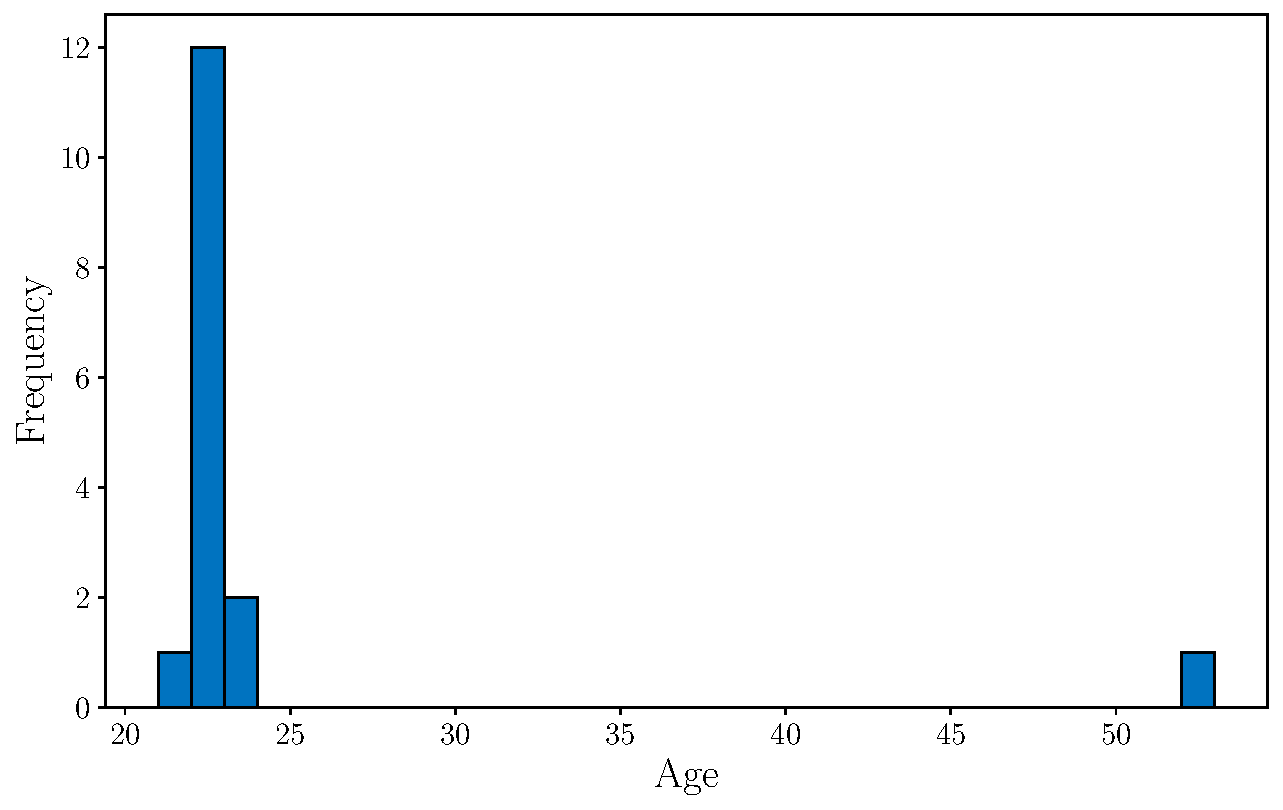
\includegraphics{./evaluation/figures/survery/age-distribution.pdf}
	  }
	}
	\hfill
	\pictureBox[label={fig:incorrect-head-track}]{Glasses}{
	\adjustbox{height=6cm, keepaspectratio}{
	  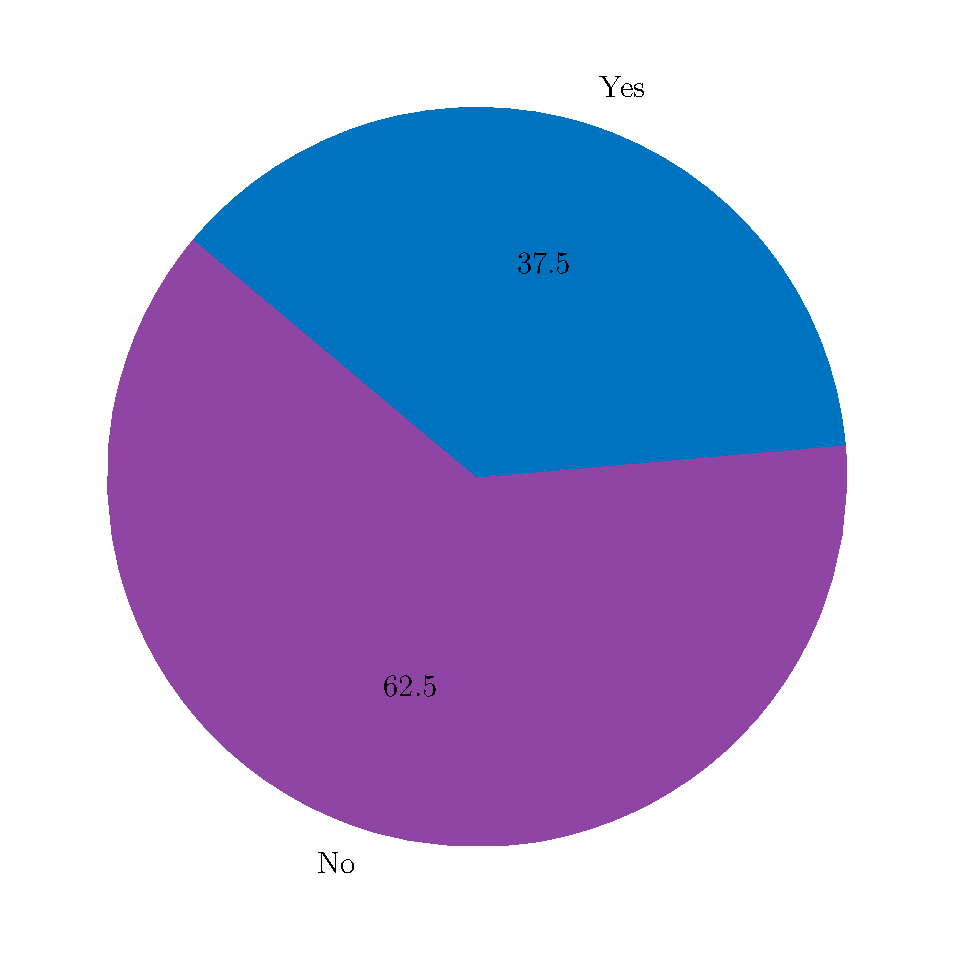
\includegraphics{./evaluation/figures/survery/glasses-distribution.pdf}
	  }
	}
	\\
	\pictureBox[label={fig:head-angle}]{Used VR/AR}{
	  \adjustbox{height=7.75cm, keepaspectratio}{
		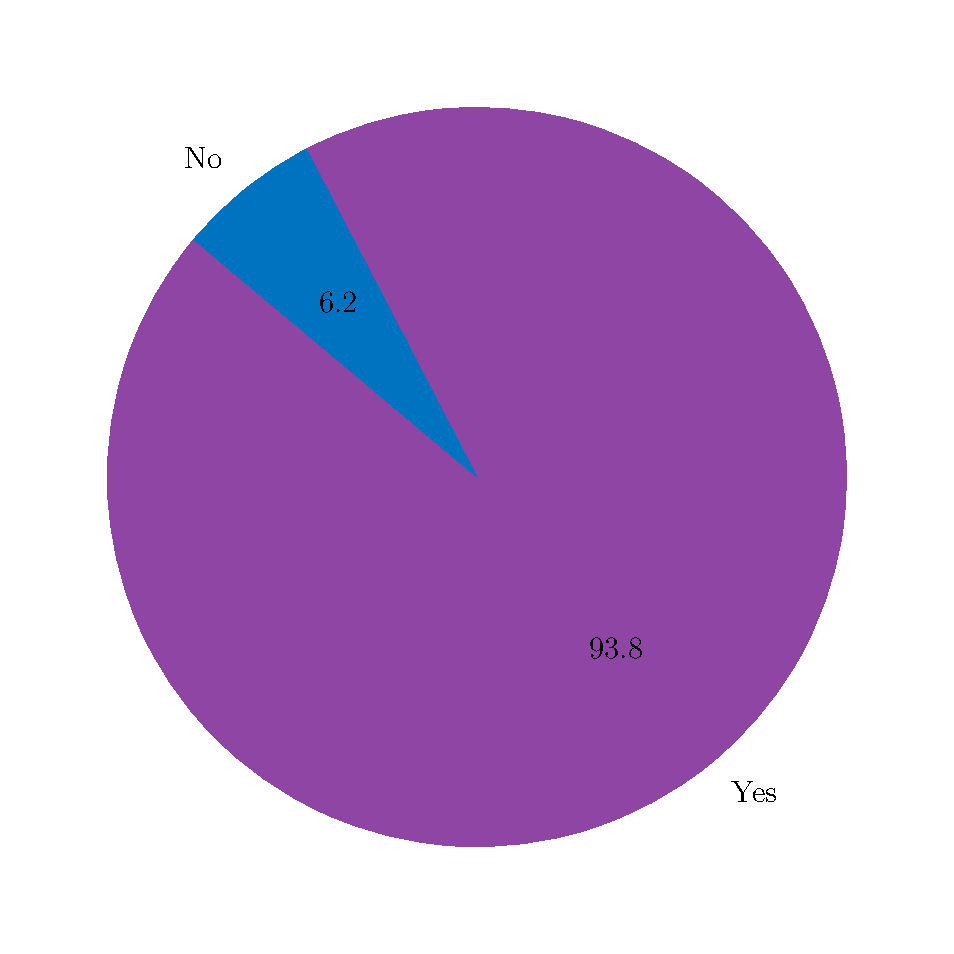
\includegraphics{./evaluation/figures/survery/vr-ar-distribution.pdf}
	  }
	}
	\hfill
	\pictureBox[label={fig:incorrect-head-track}]{Gender}{
	\adjustbox{height=7.75cm, keepaspectratio}{
	  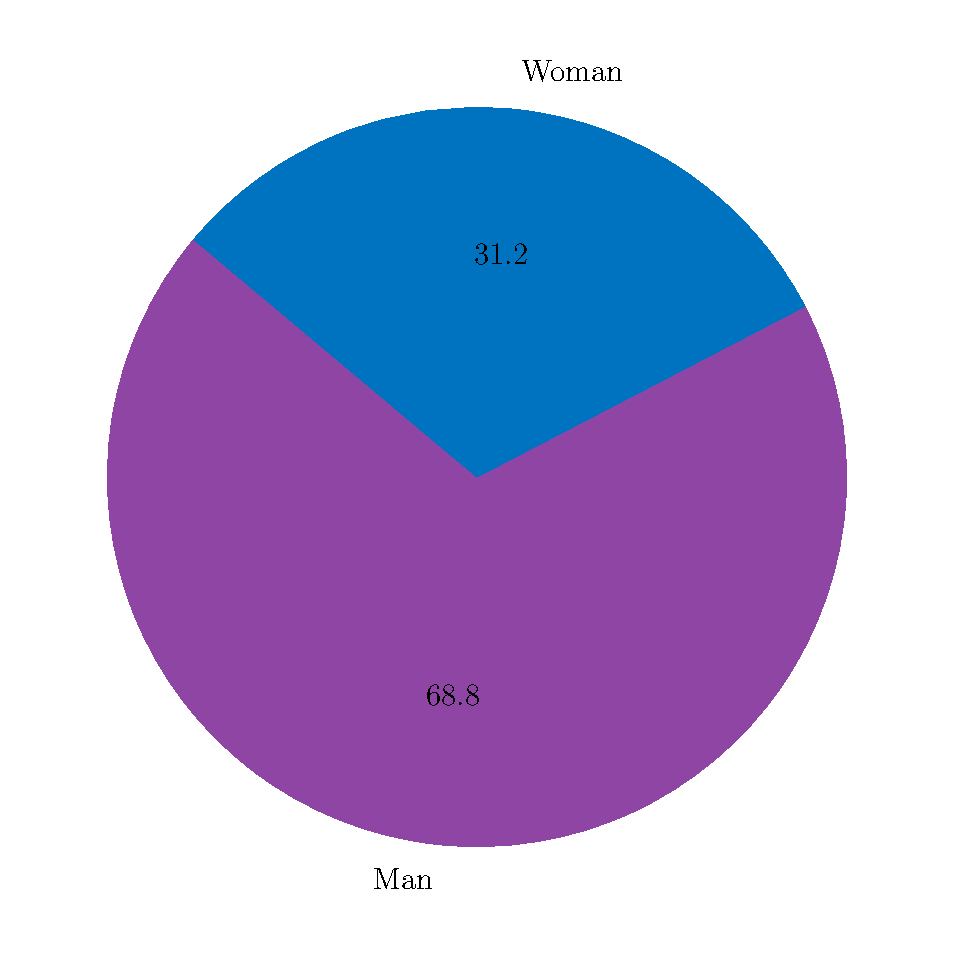
\includegraphics{./evaluation/figures/survery/gender-distribution.pdf}
	  }
	}
\end{invisBox}

\subsection{Survey Results}

When asked to rank the conditions they undertook in order of preferences people overwhelmingly seemed to prefer the Tracker conditions as can be seen in \ref{fig:condition-preferences}. Only 13\% of people picked either of the Static conditions as their first choice. \textcolor{red}{write more and provide some analysis} 

\begin{figureBox}[label={fig:condition-preferences}, width=1.0\linewidth]{Study Condition Rankings}
    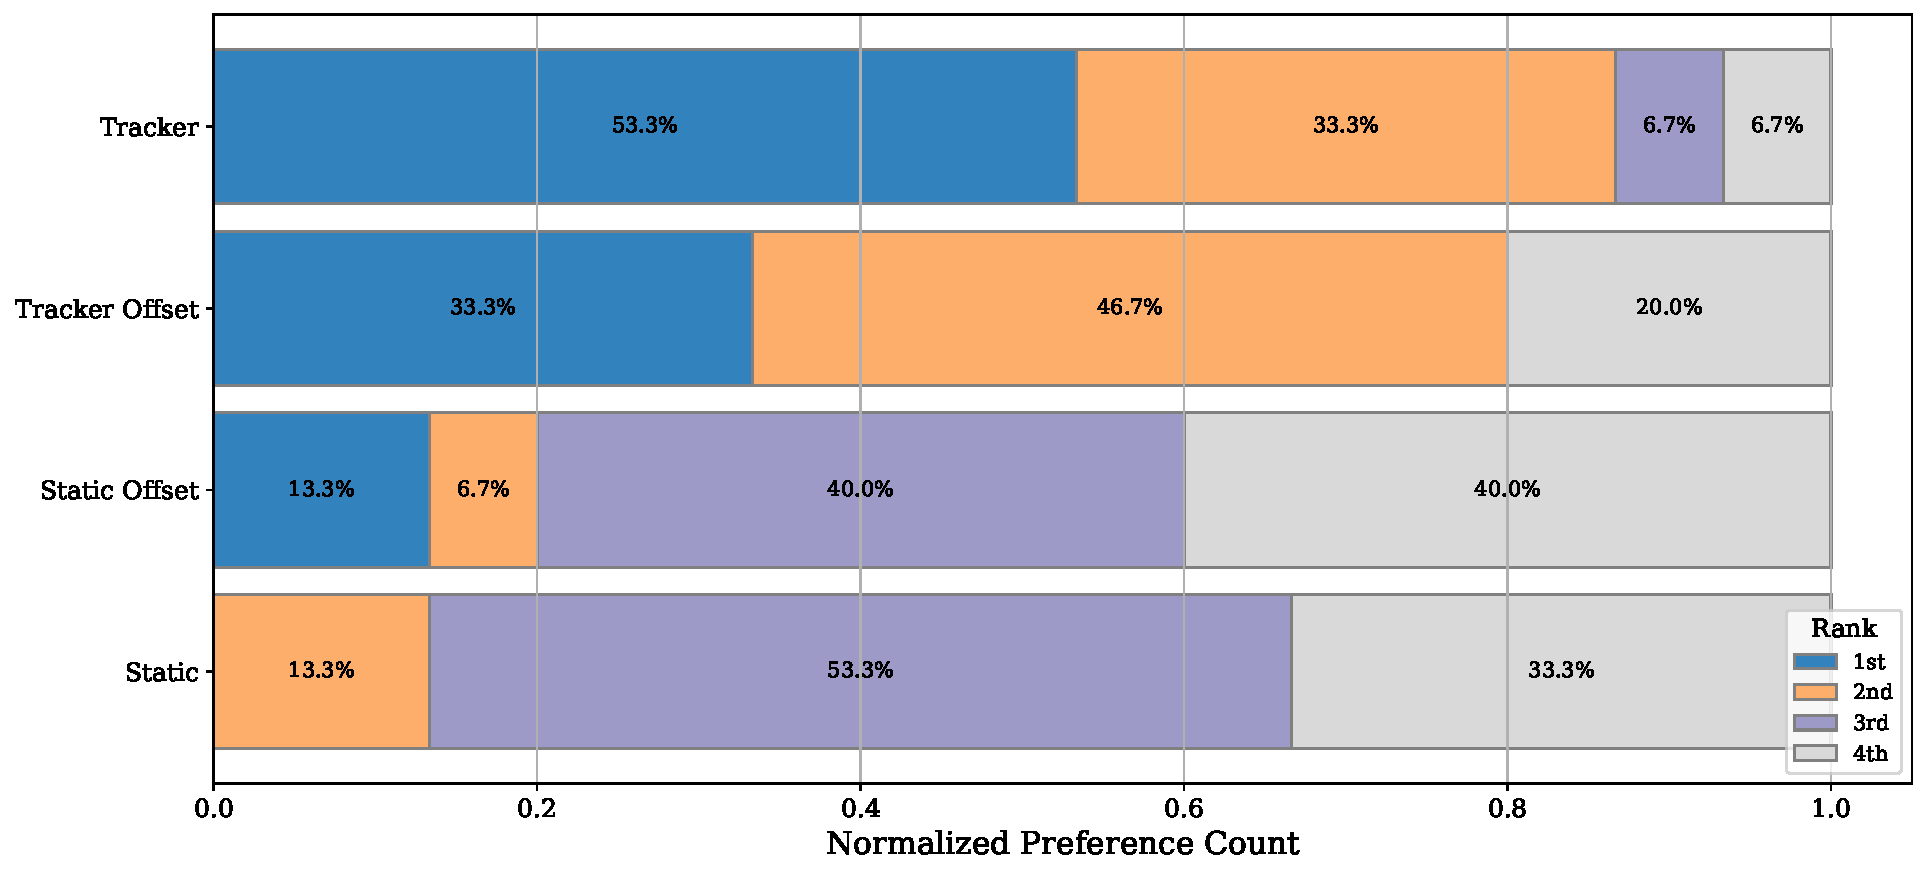
\includegraphics[width = 1.0\linewidth]{./evaluation/figures/survery/preferences.pdf}
\end{figureBox}

Unsurprisingly people found the head tracking more reliable when compared to the head track as can be seen in \ref{fig:reliable}. This is backed out by the fail rates we observed in both systems as can be seen in \textcolor{red}{insert other figure currently in system, maybe move it to this study section?}

\begin{figureBox}[label={fig:reliable}, width=0.8\linewidth]{Mean Accuracy and Reliability of Hand and Eye Tracking}
    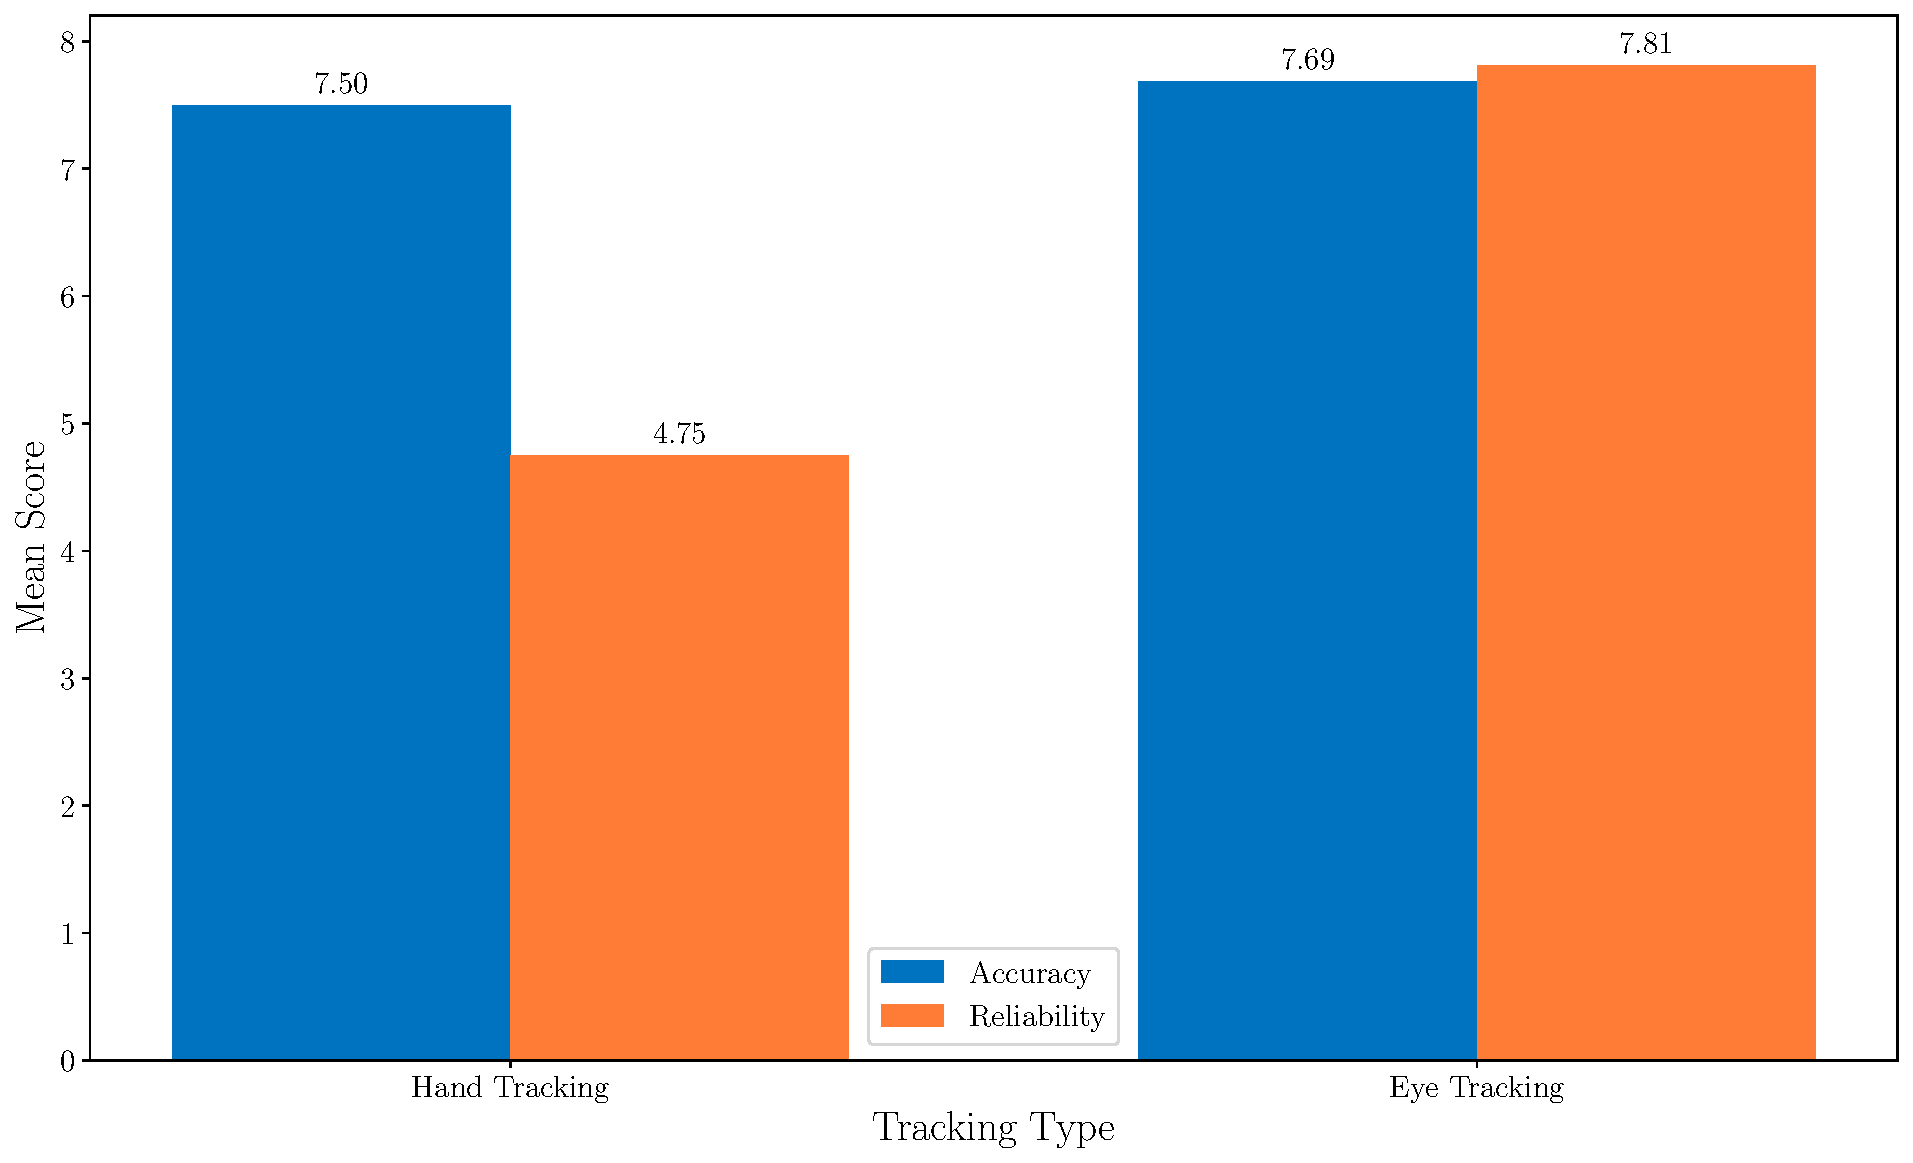
\includegraphics[width = 1.0\linewidth]{./evaluation/figures/survery/reliable-accurate.pdf}
\end{figureBox}

\subsection{Data results}

We analysed the time taken to complete each segment of each task and found that the type of view and the offset had a significant effect on the time taken to complete the segment. This can be seen in \ref{fig:anova-interaction}. \\

\begin{figureBox}[label={fig:anova-interaction}, width=0.8\linewidth]{Interaction between Type and Offset of segment times}
    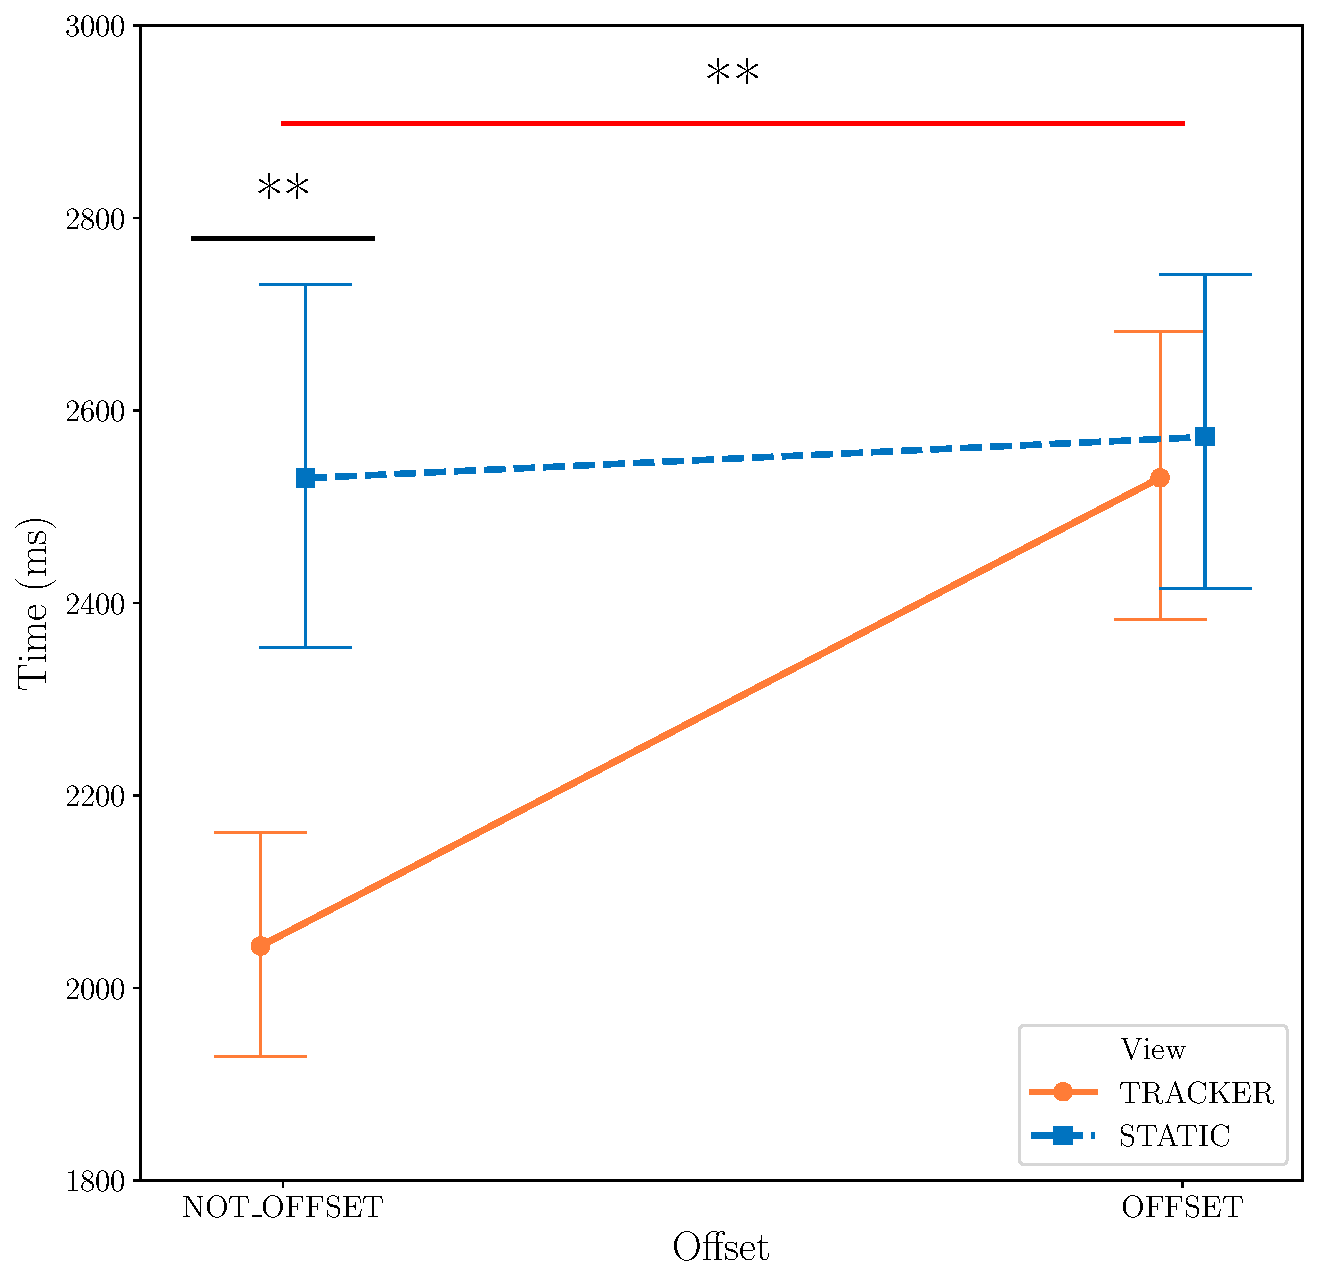
\includegraphics[width = 1.0\linewidth]{./evaluation/figures/survery/anova-interaction.pdf}
\end{figureBox}

We ran a type 2 anova test to verify that these results are indeed significant as can be seen in Table~\ref{tab:anova}. 

\begin{table}[h!]
	\centering
	\caption{ANOVA Table for Fig~\ref{fig:anova-interaction}}
	\label{tab:anova}
	\begin{tabular}{lS[table-format=1.2e+2]S[table-format=4.0]S[table-format=2.6]S[table-format=1.6]}
		\toprule
		\textbf{Source} & \textbf{Sum of Squares} & \textbf{df} & \textbf{F} & \textbf{p-value} \\
		\midrule
		\texttt{C(Type)} & 3.363186e+07 & 1.0 & 10.698212 & 0.001092 \\
		\texttt{C(Offset)} & 3.341680e+07 & 1.0 & 10.629800 & 0.001132 \\
		\texttt{C(Type):C(Offset)} & 2.344484e+07 & 1.0 & 7.457744 & 0.006375 \\
		\texttt{Residual} & 5.985586e+09 & 1904.0 & NaN & NaN \\
		\bottomrule
	\end{tabular}
\end{table}

People were best at completing the segments when using the TRACKER mode (3D view) directly in front of them. They approximately equally bad at completing all other conditions. This implies the 3D view is only really useful when directly in front of you. This is understandable as the further an object is away the less information you can get from it by moving your head. Interestingly we found that users still moved their head the same amount regardless of the view type as can be seen in Fig~\ref{fig:eye-movement}.


\begin{figureBox}[label={fig:eye-movement}, width=0.8\linewidth]{Combined Mean Eye Movement Values Per Millisecond and Standard Deviations}
    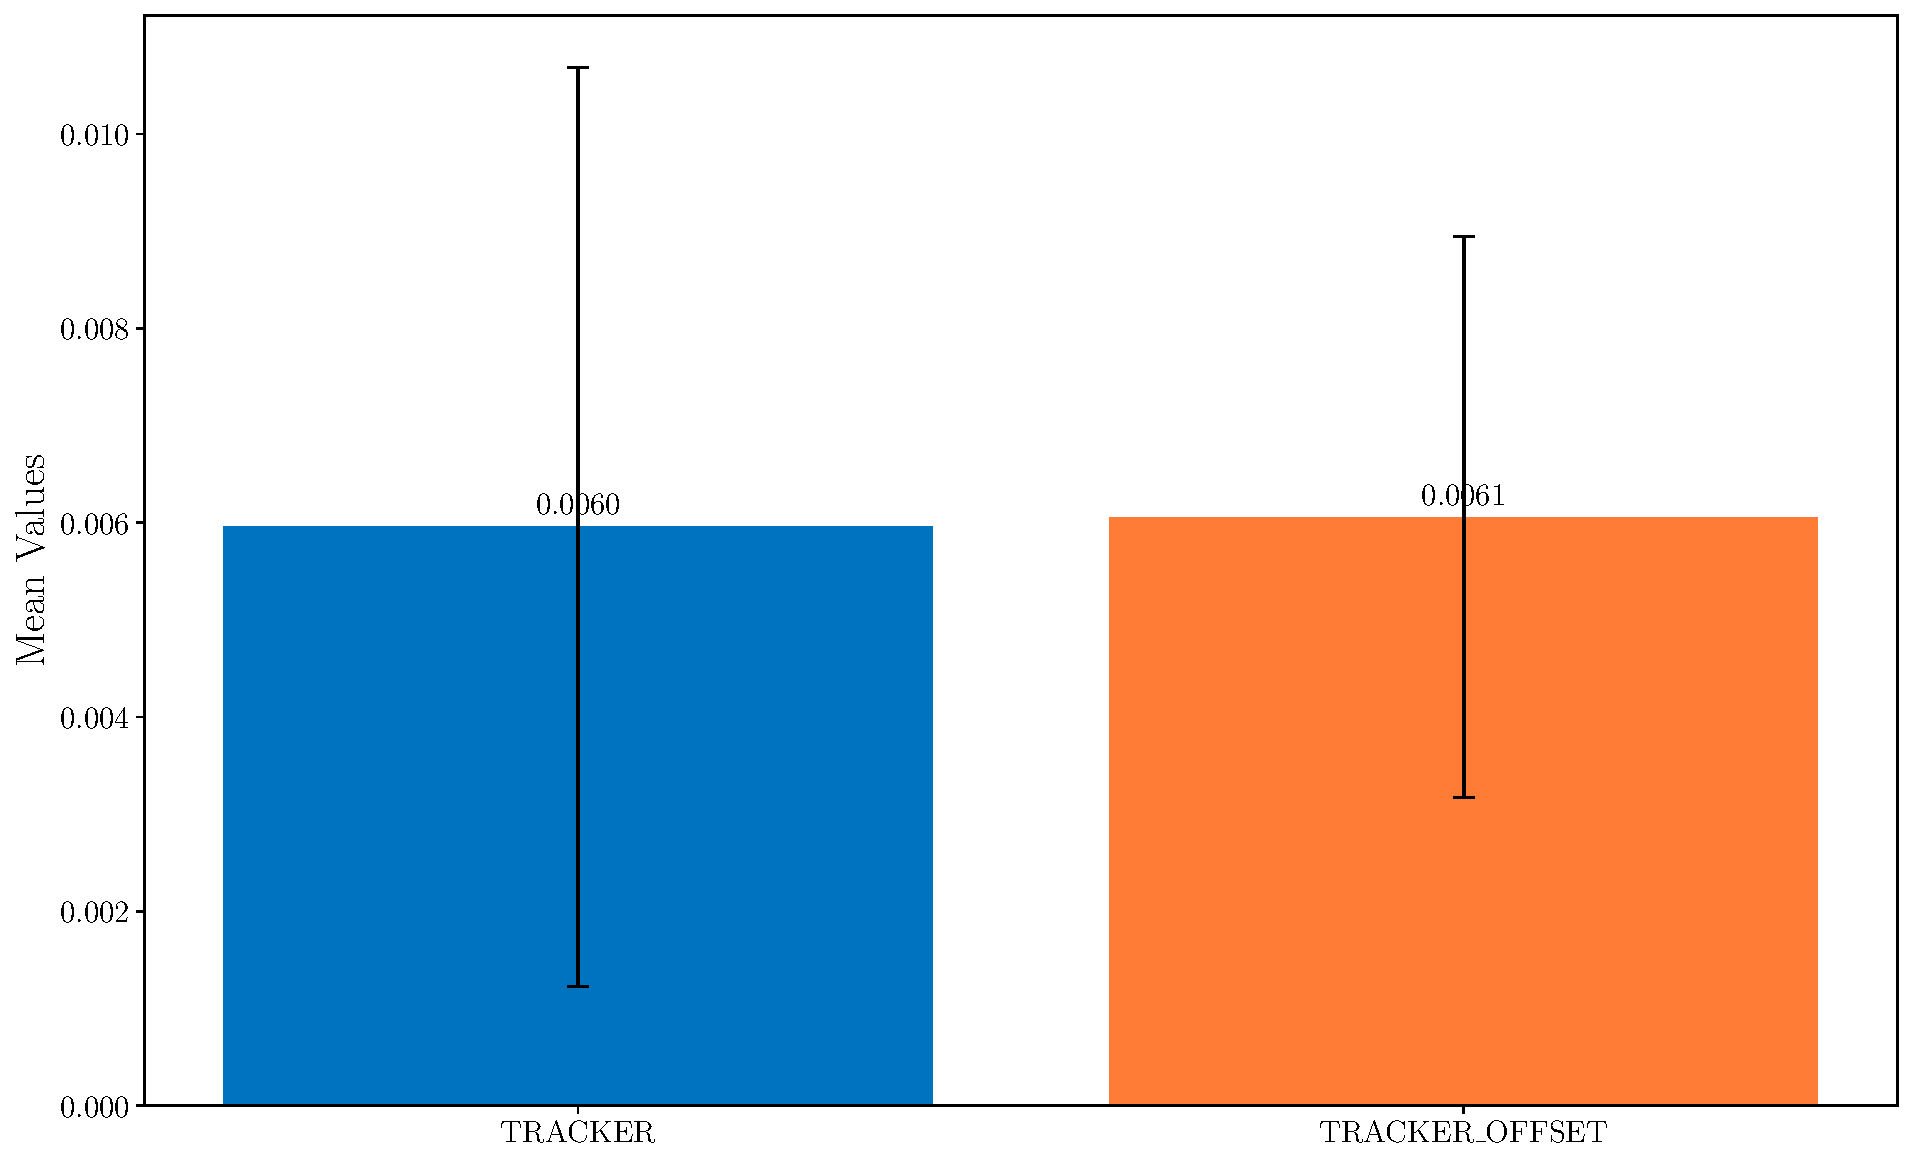
\includegraphics[width = 1.0\linewidth]{./evaluation/figures/survery/combined-eye-movement.pdf}
\end{figureBox}

As can be seen from Table~\ref{tab:ttest} the t-test we ran suggests the offset condition does not have a significant effect on eye/head movement. 

\begin{table}[h!]
    \centering
    \caption{T-Test Result for Fig~\ref{fig:eye-movement}}
    \label{tab:ttest}
    \begin{tabular}{lS[table-format=2.4]S[table-format=1.6]}
        \toprule
        \textbf{Statistic} & \textbf{Value} & \textbf{p-value} \\
        \midrule
        \texttt{T-statistic} & -0.4170 & 0.6767 \\
        \bottomrule
    \end{tabular}
\end{table}
Interestingly the data seems to suggest that offset interaction does not have a significant effect on the time taken to complete the segment. This is surprising as we expected the offset to have a significant effect on the time taken to complete the segment. One people reason might be the downside of the offset might be accounted for by the fact the participants hands no longer occlude their view of the scene. \\

One study we would like to run in the future is to see what happens if we offset the interaction zone instead of the view, this would control for the apparent factor that 3D is less useful far away.  

\begin{enumerate}
	\item For each task graph the distance of the points to it, see if people spend more time trying to be exactly precise.
	\item Look at overall head movement, see if people are moving their head more in TRACKER vs TRACKER\_OFFSET
\end{enumerate}

\textcolor{red}{Add more graphs in the appendix and talk about them here, put the task side by side with the results}